\documentclass[usenames,dvipsnames,aspectratio=169]{beamer}
\usepackage{../common/prgBasics}

\title[Lecture 10.]{Programming basics}
\subtitle{(GKNB\_INTA023)}

\begin{document}

%1
\begin{frame}[plain]
  \titlepage
\end{frame}

%2
\begin{frame}{Macros with arguments}
  Problem:
  \begin{itemize}
    \item[] If a function is very simple, the \emph{time of invocation} is comparable with the \emph{time of operation} $\to$ ineffectice, slow programs
  \end{itemize}
  Solution:
  \begin{itemize}
    \item[] Change function calls to macro substitution! $\to$ text replacement with the preprocessor
  \end{itemize}
\end{frame}

%3
\begin{frame}{Macros with arguments}
  \footnotesize
  \begin{exampleblock}{\textattachfile{operation1.c}{operation1.c}}
    \lstinputlisting[style=c]{operation1.c}
  \end{exampleblock}
  \vfill
  \normalsize
  Task: substitute all function calls with macros!\\
  \scriptsize 
  \texttt{\#define \emph{name}(\emph{identifier-list}) \emph{preprocessor-symbols}} \emph{newline}
\end{frame}

%4
\begin{frame}{Macros with arguments}
  \kiemel{Caution!} \\
  \small
  It is forbidden to put a whitespace character between \kiemel{\texttt{SQUARE}} and \kiemel{\texttt{(}}! $\to$ changes the meaning to simple macro substitution, without arguments
  \scriptsize
  \begin{exampleblock}{\textattachfile{operation2.c}{operation2.c}}
    \lstinputlisting[style=c]{operation2.c}
  \end{exampleblock}
  \vfill
  \normalsize
  Problem: order of operations!\\
  Solution: brackets
\end{frame}

%5
\begin{frame}{Macros with arguments}
  \scriptsize
  \begin{exampleblock}{\textattachfile{operation3.c}{operation3.c}}
    \lstinputlisting[style=c]{operation3.c}
  \end{exampleblock}
  \vfill
  \normalsize
  Next task: write a macro for addition!
\end{frame}

%6
\begin{frame}{Macros with arguments}
  \scriptsize
  \begin{exampleblock}{\textattachfile{operation4.c}{operation4.c}}
    \vspace{-.3cm}
    \lstinputlisting[style=c,linerange={3-18},firstnumber=3]{operation4.c}
    \vspace{-.3cm}
  \end{exampleblock}
  \vfill
  Problem: actual parameters are evaluated before function invocation, but are used without any modifications in case of macros $\to$ different program behavior, misleading\\
  Solution: further brackets
\end{frame}

%7
\begin{frame}{Macros with arguments}
  \scriptsize
  \begin{exampleblock}{\textattachfile{operation5.c}{operation5.c}}
    \lstinputlisting[style=c,linerange={3-18},firstnumber=3]{operation5.c}
  \end{exampleblock}
\end{frame}

%8
\begin{frame}{Macros with arguments}
  Task: modify our earlier matrix addition program to calculate indexes with a macro!
  \scriptsize
  \begin{exampleblock}{\textattachfile{mtxAdd5.c}{mtxAdd5.c}}
    \lstinputlisting[style=c,linerange={5-19},firstnumber=5]{mtxAdd5.c}
  \end{exampleblock}
\end{frame}

%9
\begin{frame}{Macros with arguments}
  Pros:
  \begin{itemize}
    \item Faster than a function call
    \item The code is less type-dependent
  \end{itemize}
  \vfill
  Cons:
  \begin{itemize}
    \item No type checks, hard to explore mistakes
    \item Code size increases, it is not suitable to replace complex functions
    \item The evaluation of passed expressions happens several times $\to$ time, side effects
  \end{itemize}
\end{frame}

%10
\begin{frame}{Sorting names}
  Task:
  \begin{itemize}
    \item Read names and list them in alphabetical order!
    \item For the sake of simplicity, store the characters of names in a two-dimensional array
  \end{itemize}
  \begin{center}
    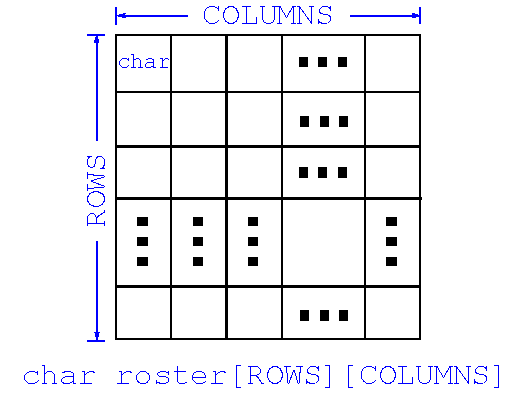
\includegraphics[scale=0.75]{roster1.pdf}
  \end{center}
\end{frame}

%11
\begin{frame}{Sorting names}
  \begin{exampleblock}{\textattachfile{roster1.c}{roster1.c}}
    \lstinputlisting[style=c,linerange={4-5},firstnumber=4]{roster1.c}
    \lstinputlisting[style=c,linerange={47-55},firstnumber=47]{roster1.c}
  \end{exampleblock}
\end{frame}

%12
\begin{frame}{Sorting names}
  \begin{exampleblock}{\textattachfile{roster1.c}{roster1.c}}
    \lstinputlisting[style=c,linerange={16-26},firstnumber=16]{roster1.c}
  \end{exampleblock}
\end{frame}

%13
\begin{frame}{Sorting names}
  \begin{exampleblock}{\textattachfile{roster1.c}{roster1.c}}
    \lstinputlisting[style=c,linerange={28-39},firstnumber=28]{roster1.c}
  \end{exampleblock}
\end{frame}

%14
\begin{frame}{Sorting names}
  \begin{exampleblock}{\textattachfile{roster1.c}{roster1.c}}
    \lstinputlisting[style=c,linerange={41-45},firstnumber=41]{roster1.c}
  \end{exampleblock}
\end{frame}

% %15
% \begin{frame}{Nevek rendezése}
%   Probléma:
%   \begin{itemize}
%     \item[] A sorok hossza azonos $\to$ néha több memóriára lenne szükség, máskor ez is túl sok
%   \end{itemize}
%   Feladat:
%   \begin{itemize}
%     \item[] Alakítsuk át az adatszerkezetet, használjunk karakteres mutatótömböt, és a soroknak foglaljunk memóriát futásidőben!
%   \end{itemize}
%   \begin{center}
%     \includegraphics[scale=0.6]{nevsor2.pdf}
%   \end{center}
% \end{frame}

% %16
% \begin{frame}{Nevek rendezése}
%   \begin{exampleblock}{\textattachfile{nevsor2.c}{nevsor2.c}}
%     \lstinputlisting[style=c,linerange={5-5},numbers=left,firstnumber=5]{nevsor2.c}
%     \lstinputlisting[style=c,linerange={56-65},numbers=left,firstnumber=56]{nevsor2.c}
%   \end{exampleblock}
% \end{frame}

% %17
% \begin{frame}{Nevek rendezése}
%   \footnotesize
%   \begin{exampleblock}{\textattachfile{nevsor2.c}{nevsor2.c}}
%     \lstinputlisting[style=c,linerange={16-30},numbers=left,firstnumber=16]{nevsor2.c}
%   \end{exampleblock}
% \end{frame}

% %18
% \begin{frame}{Nevek rendezése}
%   \footnotesize
%   \begin{exampleblock}{\textattachfile{nevsor2.c}{nevsor2.c}}
%     \lstinputlisting[style=c,linerange={32-42},numbers=left,firstnumber=32]{nevsor2.c}
%     \lstinputlisting[style=c,linerange={50-54},numbers=left,firstnumber=50]{nevsor2.c}
%   \end{exampleblock}
% \end{frame}

% %19
% \begin{frame}{Nevek rendezése}
%   Probléma:
%   \begin{itemize}
%     \item[] A nevek száma még mindig korlátozott.
%   \end{itemize}
%   Feladat:
%   \begin{itemize}
%     \item[] Foglaljunk a mutatótömbnek is memóriát futásidőben!
%   \end{itemize}
%   \footnotesize
%   \begin{exampleblock}{\textattachfile{nevsor3.c}{nevsor3.c}}
%     \lstinputlisting[style=c,linerange={56-65},numbers=left,firstnumber=56]{nevsor3.c}
%   \end{exampleblock}
% \end{frame}

% %20
% \begin{frame}{Nevek rendezése}
%   \footnotesize
%   \begin{exampleblock}{\textattachfile{nevsor3.c}{nevsor3.c}}
%     \lstinputlisting[style=c,linerange={15-29},numbers=left,firstnumber=15]{nevsor3.c}
%   \end{exampleblock}
% \end{frame}

% %21
% \begin{frame}{Nevek rendezése}
%   \footnotesize
%   \begin{exampleblock}{\textattachfile{nevsor3.c}{nevsor3.c}}
%     \lstinputlisting[style=c,linerange={43-54},numbers=left,firstnumber=43]{nevsor3.c}
%   \end{exampleblock}
% \end{frame}

% %22
% \begin{frame}{Városok közötti távolság}
%   Feladat:
%   \begin{itemize}
%     \item két város nevének beolvasása,
%     \item városok közötti távolság megjelenítése.
%     \item Kilépés azonos városok megadása esetén.
%   \end{itemize}
%   \vfill
%   Megoldás:
%   \begin{itemize}
%     \item városok nevét vektorban tároljuk
%     \item a városok közötti távolságokat pedig mátrixban, és
%     \item a városok vektorbeli indexével indexeljük a mátrixot is
%   \end{itemize}
% \end{frame}

% %23
% \begin{frame}[fragile]{Városok közötti távolság}
%   \begin{block}{Kimenet}
%     \begin{verbatim}
% Varosok kozotti tavolsag kiszamitasa
% Kilepes azonos varosok megadasaval.
% Indulo varos: Budapest
% Erkezesi varos: Salakszentmotoros
% Nem letezo varos!
% Gyor
% Tavolsag: 121km
% Indulo varos: Gyor
% Erkezesi varos: Gyor
% \end{verbatim}
%   \end{block}
% \end{frame}

% %24
% \begin{frame}{Városok közötti távolság}
%   \begin{exampleblock}{\textattachfile{varosok1.c}{varosok1.c}}
%     \footnotesize
%     \lstinputlisting[style=c,linerange={48-60},numbers=left,firstnumber=48]{varosok1.c}
%   \end{exampleblock}
% \end{frame}

% %25
% \begin{frame}{Városok közötti távolság}
%   \begin{exampleblock}{\textattachfile{varosok1.c}{varosok1.c}}
%     \scriptsize
%     \lstinputlisting[style=c,linerange={15-33},numbers=left,firstnumber=15]{varosok1.c}
%   \end{exampleblock}
% \end{frame}

% %26
% \begin{frame}{Városok közötti távolság}
%   \begin{exampleblock}{\textattachfile{varosok1.c}{varosok1.c}}
%     \lstinputlisting[style=c,linerange={35-46},numbers=left,firstnumber=35]{varosok1.c}
%   \end{exampleblock}
% \end{frame}

% %27
% \begin{frame}{Háromszögmátrixok}
%   Észrevétel: a mátrixnak több, mint fele elhagyható!\\
%   \qquad ($m_{i,j}=m_{j,i}, m_{i,i} = 0$)
%   \begin{center}
%     \small
%     \begin{tabular}{r|ccccccc}
%                   & \rotatebox{90}{Budapest} & \rotatebox{90}{Győr} & \rotatebox{90}{Szeged} &
%                     \rotatebox{90}{Debrecen} & \rotatebox{90}{Veszprém} & \rotatebox{90}{Dunaújváros} &
%                     \rotatebox{90}{Eger} \\ \hline
%       Budapest    & \kiemelZ{0}  & 121 & 174 & 231 & 115 &  83 & 139 \\
%       Győr        & \kiemel{121} & \kiemelZ{0}  & 287 & 377 &  82 & 176 & 285 \\
%       Szeged      & \kiemel{174} & \kiemel{287} & \kiemelZ{0}  & 218 & 278 & 161 & 298 \\
%       Debrecen    & \kiemel{231} & \kiemel{377} & \kiemel{218} & \kiemelZ{0}  & 368 & 320 & 131 \\
%       Veszprém    & \kiemel{115} & \kiemel{82}  & \kiemel{278} & \kiemel{368} & \kiemelZ{0}  & 103 & 275 \\
%       Dunaújváros & \kiemel{83}  & \kiemel{176} & \kiemel{161} & \kiemel{320} & \kiemel{103} & \kiemelZ{0}  & 228 \\
%       Eger        & \kiemel{139} & \kiemel{285} & \kiemel{298} & \kiemel{131} & \kiemel{275} & \kiemel{228} & \kiemelZ{0} \\
%     \end{tabular}
%   \end{center}
%   Probléma: a mátrixnak minden sora azonos elemszámú\\
%   Megoldás: eltérő elemszámú vektorokat címző vektor létrehozása\\
%   \qquad (mutatótömb, alsó háromszögmátrix)
% \end{frame}

% %28
% \begin{frame}{Háromszögmátrixok}
%   \begin{exampleblock}{\textattachfile{varosok2.c}{varosok2.c}}
%     \footnotesize
%     \lstinputlisting[style=c,linerange={35-50},numbers=left,firstnumber=24]{varosok2.c}
%   \end{exampleblock}
% \end{frame}

% %29
% \begin{frame}{Alternatív megoldás}
%   Észrevétel: még a vektorokat címző mutatók is megtakaríthatók, ha sorfolytonosan, egyetlen vektorban tároljuk a főátló alatti 
% értékeket!
%   \begin{center}
%     \scriptsize
%     \begin{tabular}{r|cccccc}
%                   & \rotatebox{90}{Bp. [0]} & \rotatebox{90}{Győr [1]} & \rotatebox{90}{Szeged [2]} &
%                     \rotatebox{90}{Debr. [3]} & \rotatebox{90}{Veszp. [4]} & \rotatebox{90}{Duv. [5]}\\ \hline
%       Győr [1]        & \kiemelZ{121} & & & & & \\
%       Szeged [2]      & \kiemelZ{174} & \kiemelZ{287} & & & & \\
%       Debrecen [3]    & \kiemelZ{231} & \kiemelZ{377} & \kiemelZ{218} & & & \\
%       Veszprém [4]    & \kiemel{115} & \kiemel{82} & 278 & 368 & & \\
%       Dunaújváros [5] & 83 & 176 & 161 & 320 & 103 & \\
%       Eger [6]        & 139 & 285 & 298 & 131 & 275 & 228 \\
%     \end{tabular}\\
%     \vspace{.3cm}
%     \begin{tabular}{c|cc|ccc|cccc}
%       [0] & [1] & [2] & [3] & [4] & [5] & [6] & [7] & [8] & [9] \\ \hline
%       \kiemelZ{121} & \kiemelZ{174} & \kiemelZ{287} & \kiemelZ{231} & \kiemelZ{377} & \kiemelZ{218} & 
%         \kiemel{115} & \kiemel{82} & 278 & \dots \\
%     \end{tabular}
%   \end{center}
%   Keresett elem feletti sorokban lévő adatok száma sorról sorra számtani sort alkot 
%   $\to S_n = \frac{[2a_1 + (n-1)d] \cdot n}{2}$, speciálisan $a_1=1, d=1 \to S_n = \frac{(n+1) \cdot n}{2}$
% \end{frame}

% %30
% \begin{frame}{Alternatív megoldás}
%   \tiny
%   Vigyázz! A programban a sorok indexelése 0-val kezdődik, nem 1-gyel!
%   \begin{exampleblock}{\textattachfile{varosok3.c}{varosok3.c}}
%     \scriptsize
%     \lstinputlisting[style=c,linerange={35-51},numbers=left,firstnumber=35]{varosok3.c}
%   \end{exampleblock}
% \end{frame}

% %31
% \begin{frame}{Statikus változók}
%   Probléma:
%   \begin{itemize}
%     \item a lokális változók alapértelmezetten \emph{automatikusak} (\texttt{auto}): élettartam a definíció pillanatától a 
% blokk elhagyásáig tart
%     \item a vektorok és tömbök újrafoglalása időigényes
%   \end{itemize}
%   \vfill
%   Megoldás: \texttt{static} minősítő használata
%   \begin{itemize}
%     \item élettartam: program indulásától leállásig $\to$ értéküket megőrzik a függvényhívások között
%     \item hatókör: változatlan (deklarációtól blokk végéig)
%     \item implicit módon inicializált (feltöltés zérus értékű bitekkel)
%   \end{itemize}
% \end{frame}

% %32
% \begin{frame}{Statikus változók}
%   \begin{exampleblock}{\textattachfile{varosok4.c}{varosok4.c}}
%     \scriptsize
%     \lstinputlisting[style=c,linerange={35-51},numbers=left,firstnumber=35]{varosok4.c}
%   \end{exampleblock}
% \end{frame}

% %33
% \begin{frame}{Dinamikus háromszögmátrixok}
%   Feladat: 
%   \begin{itemize}
%     \item hozzuk létre futásidőben a vektort és a háromszögmátrixot!
%     \item töltsük fel őket felhasználó által adott értékekkel!
%   \end{itemize}
%   \begin{exampleblock}{\textattachfile{varosok5.c}{varosok5.c} -- \texttt{main}}
%     \scriptsize
%     \lstinputlisting[style=c,linerange={77-88},numbers=left,firstnumber=77]{varosok5.c}
%   \end{exampleblock}
% \end{frame}

% %34
% \begin{frame}{Dinamikus háromszögmátrixok}
%   \begin{exampleblock}{\textattachfile{varosok5.c}{varosok5.c} -- \texttt{main}}
%     \footnotesize
%     \lstinputlisting[style=c,linerange={89-101},numbers=left,firstnumber=89]{varosok5.c}
%   \end{exampleblock}
% \end{frame}

% %35
% \begin{frame}{Dinamikus háromszögmátrixok}
%   \small
%   \begin{exampleblock}{\textattachfile{varosok5.c}{varosok5.c}}
%     \lstinputlisting[style=c,linerange={16-27},numbers=left,firstnumber=16]{varosok5.c}
%   \end{exampleblock}
% \end{frame}

% %36
% \begin{frame}{Dinamikus háromszögmátrixok}
%   \begin{exampleblock}{\textattachfile{varosok5.c}{varosok5.c}}
%     \lstinputlisting[style=c,linerange={43-54},numbers=left,firstnumber=43]{varosok5.c}
%   \end{exampleblock}
% \end{frame}

% %37
% \begin{frame}{Dinamikus háromszögmátrixok}
%   \footnotesize
%   \begin{exampleblock}{\textattachfile{varosok5.c}{varosok5.c}}
%     \lstinputlisting[style=c,linerange={29-41},numbers=left,firstnumber=29]{varosok5.c}
%   \end{exampleblock}
% \end{frame}

% %38
% \begin{frame}{Dinamikus háromszögmátrixok}
%   \begin{exampleblock}{\textattachfile{varosok5.c}{varosok5.c}}
%     \lstinputlisting[style=c,linerange={56-64},numbers=left,firstnumber=56]{varosok5.c}
%   \end{exampleblock}
% \end{frame}

% %39
% \begin{frame}{Dinamikus háromszögmátrixok}
%   \begin{exampleblock}{\textattachfile{varosok5.c}{varosok5.c}}
%     \lstinputlisting[style=c,linerange={66-75},numbers=left,firstnumber=66]{varosok5.c}
%   \end{exampleblock}
% \end{frame}

% %40
% \begin{frame}{Bűvös négyzet (magic square)}
%   \begin{itemize}
%     \item Olyan (ált. 1 és $n^2$ közötti) egész számokat tartalmazó négyzetes mátrix, melynek
%     \begin{itemize}
%       \item minden sorösszege,
%       \item minden oszlopösszege,
%       \item főátlójában és
%       \item mellékátlójában lévő számok összege azonos.
%     \end{itemize}
%     \item \hiv{\href{http://en.wikipedia.org/wiki/Magic_square}{További érdekességek}}
%   \end{itemize}
%   \begin{center}
%     \tiny
%     \begin{tabular}{cc}
%       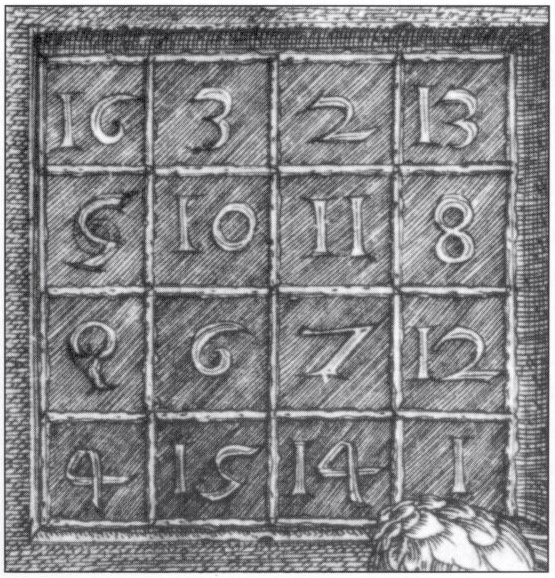
\includegraphics[height=3cm]{melancolia.jpg} & 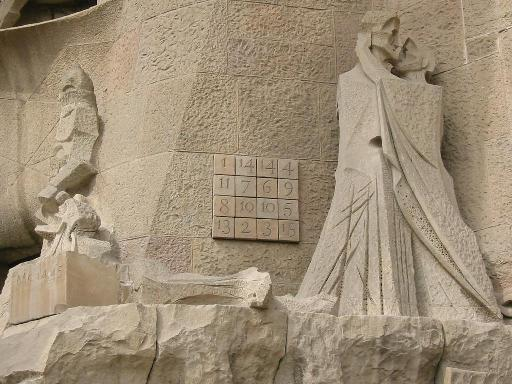
\includegraphics[height=3cm]{sagrada.jpg} \\
%       Albrecht Dürer: Melencolia I (részlet) & Sagrada Família, Barcelona\\
%     \end{tabular}
%   \end{center}
% \end{frame}

% %41
% \begin{frame}{Bűvös négyzet (magic square)}
%   \scriptsize
%  \hiv{\href
%  {http://en.wikipedia.org/wiki/Magic_square\#Method_for_constructing_a_magic_square_of_odd_order}
%  {Páratlan rendű bűvös négyzetek konstrukciója}}
%   \begin{enumerate}
%     \item A mátrix első sorának középső oszlopába írjunk 1-et!
%     \item A mátrix minden további elemének értéke legyen eggyel nagyobb a korábbinál (2, 3, \dots,
% $n^2$)!
%     \item A következő elemet úgy választjuk ki, hogy \kiemel{jobbra és felfelé} lépünk egyet.
%     \begin{itemize}
%       \scriptsize
%       \item Ha a meghatározott elem már korábban ki lett töltve, akkor az utoljára kitöltött elem
% \kiemel{alatti} elemmel kell folytatni a műveletet.
%       \item Ha az így meghatározott elem kívül esne a mátrixon, akkor a szemközti oldalon lévő első
% elemet kell használni (pl. a ,,legfelső feletti'' sor esetén a legalsót).
%     \end{itemize}
%   \end{enumerate}
%   \begin{center}
%     \begin{tabular}{|C{.2cm}|C{.2cm}|C{.2cm}|}
%       \hline
%       \multicolumn{3}{|c|}{1. lépés}\\
%       \hline
%        & 1 &  \\
%       \hline
%        &  &  \\
%       \hline
%        &  &  \\
%       \hline
%     \end{tabular}
%     \begin{tabular}{|C{.2cm}|C{.2cm}|C{.2cm}|}
%       \hline
%       \multicolumn{3}{|c|}{2. lépés}\\
%       \hline
%        & 1 &  \\
%       \hline
%        &  &  \\
%       \hline
%        &  & 2 \\
%       \hline
%     \end{tabular}
%     \begin{tabular}{|C{.2cm}|C{.2cm}|C{.2cm}|}
%       \hline
%       \multicolumn{3}{|c|}{3. lépés}\\
%       \hline
%        & 1 &  \\
%       \hline
%       3 &  &  \\
%       \hline
%        &  & 2 \\
%       \hline
%     \end{tabular}
%     \begin{tabular}{|C{.2cm}|C{.2cm}|C{.2cm}|}
%       \hline
%       \multicolumn{3}{|c|}{4. lépés}\\
%       \hline
%        & 1 &  \\
%       \hline
%       3 &  &  \\
%       \hline
%       4 &  & 2 \\
%       \hline
%     \end{tabular}
%     \begin{tabular}{|C{.2cm}|C{.2cm}|C{.2cm}|}
%       \hline
%       \multicolumn{3}{|c|}{5. lépés}\\
%       \hline
%        & 1 &  \\
%       \hline
%       3 & 5 &  \\
%       \hline
%       4 &  & 2 \\
%       \hline
%     \end{tabular}
%     \begin{tabular}{|C{.2cm}|C{.2cm}|C{.2cm}|}
%       \hline
%       \multicolumn{3}{|c|}{6. lépés}\\
%       \hline
%        & 1 & 6 \\
%       \hline
%       3 & 5 &  \\
%       \hline
%       4 &  & 2 \\
%       \hline
%     \end{tabular}
%     \begin{tabular}{|C{.2cm}|C{.2cm}|C{.2cm}|}
%       \hline
%       \multicolumn{3}{|c|}{7. lépés}\\
%       \hline
%        & 1 & 6 \\
%       \hline
%       3 & 5 & 7 \\
%       \hline
%       4 &  & 2 \\
%       \hline
%     \end{tabular}
%     \begin{tabular}{|C{.2cm}|C{.2cm}|C{.2cm}|}
%       \hline
%       \multicolumn{3}{|c|}{8. lépés}\\
%       \hline
%       8 & 1 & 6 \\
%       \hline
%       3 & 5 & 7 \\
%       \hline
%       4 &  & 2 \\
%       \hline
%     \end{tabular}
%     \begin{tabular}{|C{.2cm}|C{.2cm}|C{.2cm}|}
%       \hline
%       \multicolumn{3}{|c|}{9. lépés}\\
%       \hline
%       8 & 1 & 6 \\
%       \hline
%       3 & 5 & 7 \\
%       \hline
%       4 & 9 & 2 \\
%       \hline
%     \end{tabular}
%   \end{center}
% \end{frame}

% %42
% \begin{frame}{Bűvös négyzet (magic square)}
%   \begin{exampleblock}{\textattachfile{buvos.c}{buvos.c}}
%     \lstinputlisting[style=c,linerange={43-53},numbers=left,firstnumber=43]{buvos.c}
%   \end{exampleblock}
% \end{frame}

% %43
% \begin{frame}{Bűvös négyzet (magic square)}
%   \small
%   \begin{exampleblock}{\textattachfile{buvos.c}{buvos.c} -- \texttt{eloallit}}
%     \lstinputlisting[style=c,linerange={4-10},numbers=left,firstnumber=4]{buvos.c}
%   \end{exampleblock}
% \end{frame}

% %44
% \begin{frame}{Bűvös négyzet (magic square)}
%   \begin{exampleblock}{\textattachfile{buvos.c}{buvos.c} -- \texttt{eloallit}}
%     \footnotesize
%     \lstinputlisting[style=c,linerange={11-25},numbers=left,firstnumber=11]{buvos.c}
%   \end{exampleblock}
% \end{frame}

% %45
% \begin{frame}{Bűvös négyzet (magic square)}
%   \begin{exampleblock}{\textattachfile{buvos.c}{buvos.c}}
%     \footnotesize
%     \lstinputlisting[style=c,linerange={27-41},numbers=left,firstnumber=27]{buvos.c}
%   \end{exampleblock}
% \end{frame}

\end{document}
